\chapter{Predictive maintenance for electrical submersible pumps}

\section{Introduction}
As any pumping artificial lift method, \ac{ESP}s exhibit failures. The maintenance of \ac{ESP}s expends a lot of resources and manpower and is usually triggered and accompanied by the reactive process monitoring of multivariate sensor data.

In general, this chapter work focusing on the usage of machine learning to understanding an equipment status so as to facilitate predictive maintenance and to avoid operation downtime. ESPs are installed in many producing wells that are subject to harsh environments and need to pump complex fluid mixtures that on their turn undergo changes in composition, pressure and temperature over time. For assuring a reliable fluid delivery, on time interventions are required in case of upcoming problems. Hence, strong efforts are undertaken in the area of “digital oil field”, that focus on deploying machine learning and data-driven models in the area of predictive pump maintenance of electrical submersible pumps.

In this chapter, we introduce a contribution to the area of efficiency increase by reducing the time required to dismantle the system, inspect it and perform failure analysis. The objective is achieved by applying the \ac{PCA} as a dimentionality reduction technique then its output is pipelined with a model trained using\ac{XGBoosting} algorithm for future prediction of the system pre-workver events.

The proposed model is able to identify deeper functional relationships and longer-term trends inferred from historical data. The novel workflow with the predictive model can provide alarms within seven days before the actual failure event. 

\section{Data gathering and Pre-Processing}

Time series data are collected from sensors on \ac{ESP} wells. The reported measurements are \ac{FRQ}, \ac{PDP}, \ac{PIP}, \ac{WHP}, \ac{WHT}, \ac{MT}, \ac{CHP} and \ac{Current}. They have different frequencies. Also well status sheets for the same wells at the same time periods are gathered in daily frequency. These data come from a field that has a polymer flooding project. Based on the status sheets, pumps exhibits two main categories of problems. Those are \ac{MDHF} and \ac{EDHF} therefore both are laying under electrical pump failures. 

Electric Failures of the downhole facilities, both \ac{MDHF} and \ac{EDHF}, are failures of any of the electrical components in the ESP assembly including the electric cable, the motor electrical components such as the stator, and the downhole sensor. Failures associated with the electric cables are mainly caused by cable insulation due to corrosion, material failure, cable failure due to overload. While electrical failures associated with the motor are usually a resultant of the stator failure. The stator has been reported to fail due to overheating due to temperature. As the motor is the hottest point in the well, this appears to worsen polymer deposition on the motor body. This in turn reduces heat dissipation leading to increasing motor winding temperature, which in turn make the deposition worse and eventual ramp down of ESP frequency when maximum motor temperatures are reached. Likewise, the high temperatures around the motor aids on the precipitation of solid polymer in fluids flowing past the motor and are the source of polymer plugging in the pump inlet.     

The workflow in predictive modelling starts with the data cleaning process. On one hand It is important to eliminate nonphysical values (e.g., negative or enormous pressure values), remove further outliers and align units. On the other hand, it is a critical step for handling noise data while maintaining the realistic anomalies that may identify downhole problems of the pumps. 

After visual inspection of the data, a pipeline of a pre-processing strategy is created. Firstly, it starts by resampling the data using a moving median in one-hour steps. Fig \ref{fig:boxplot_before_outlier} shows the boxplot of the data after re-sampling and before outliers removal. It is obvious that some measurements include unreasonable measurements. For example, Well head temperature reaches 18500 $^{\circ}$F which is obviously error measurement. Therefore, the second step is removing outliers. It includes first removing measurements where oil production is zero then outlier removal by limits.

\begin{figure}
    \centering
    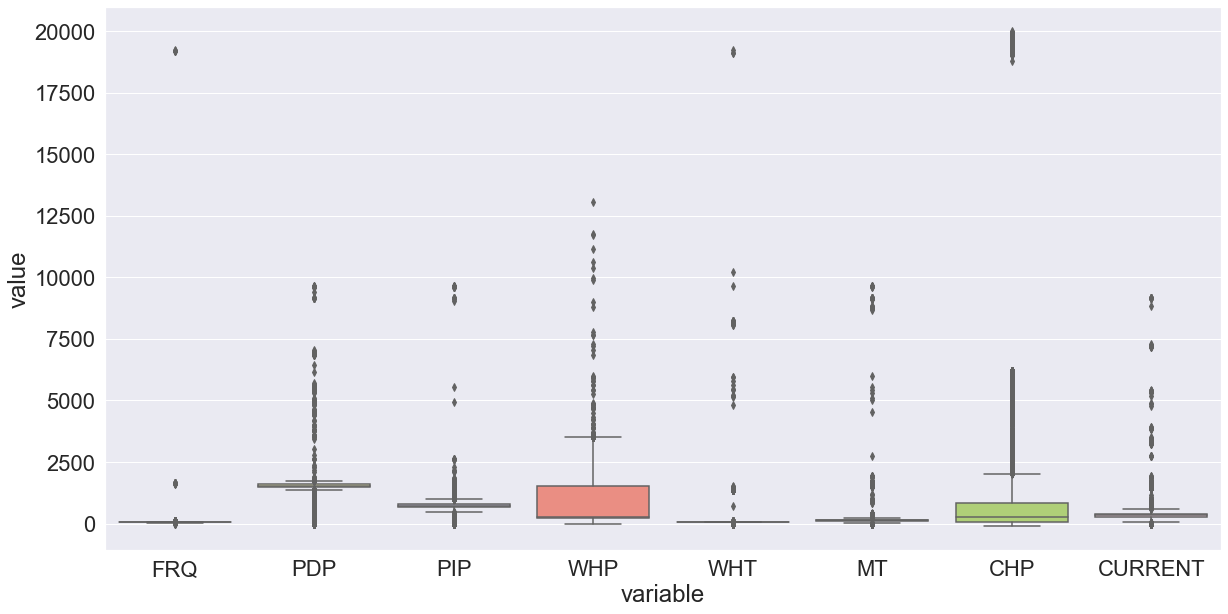
\includegraphics[width=\textwidth]{figures/predictive_maintenance/Fig 2-updates.png}
    \caption{Box-plot before outlier removal}
    \label{fig:boxplot_before_outlier}
\end{figure}

Outlier removal by limits depends mainly on quartiles therefore we used boxplots. They summarizes sample data using 25th, 50th, and 75th quartiles. The mid-spread or middle 50th, or technically H-spread, is a measure of statistical dispersion, being equal to the difference between 75th and 25th percentiles. It is called the interquartile range (IQR). IQR is somewhat similar to Z-score in terms of finding the distribution of data and then keeping some threshold to identify the outlier. To define the outlier base value is defined above and below datasets normal range namely Upper and Lower bounds. the upper and the lower bound are calculated according to equation \ref{Eq:upper_boundary} and \ref{Eq:lower_boundary}.

\begin{equation}\label{Eq:lower_boundary}
   upper = Q3 +1.5 * IQR  
\end{equation}
\begin{equation}\label{Eq:upper_boundary}
   lower = Q1 – 1.5 * IQR 
\end{equation}

Afterwards, a standard scaler is employed (subtracting mean from each point and dividing by the variance) transforming the mean value to zero and scaling the data to unit variance. Finally, the moving difference is applied on all sensors measurements. Fig. \ref{fig:boxplot_after_outlier} shows the box plot after outliers removal. Fig. \ref{fig:boxplot_after_normalization} shows the box plot after normalization.   

\begin{figure}
    \centering
    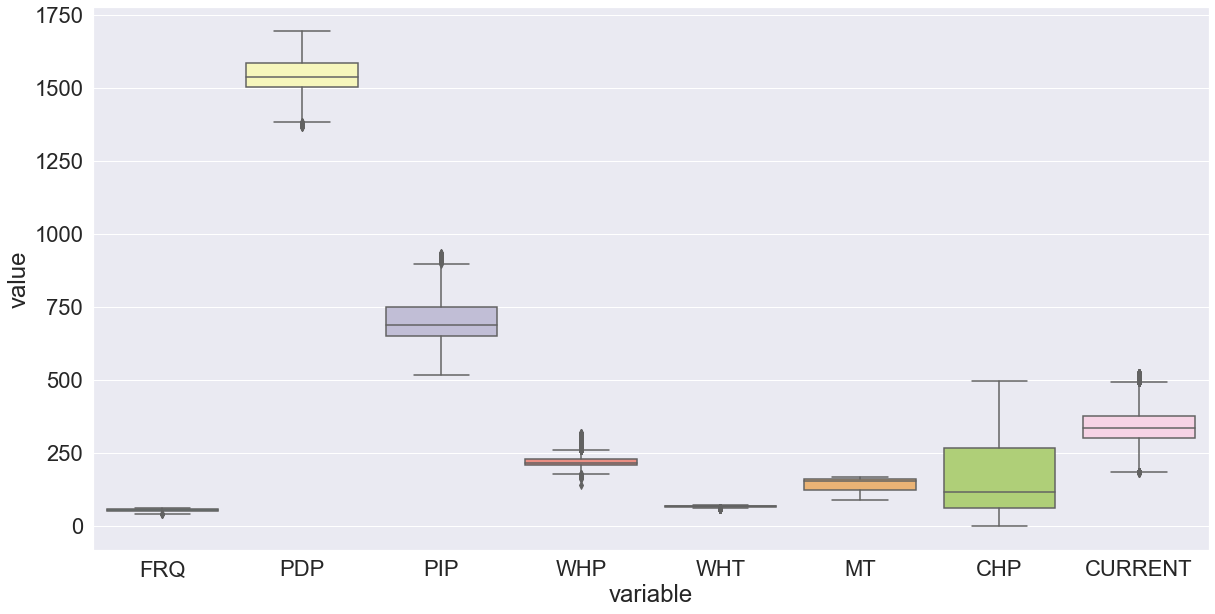
\includegraphics[width=\textwidth]{figures/predictive_maintenance/Fig 3-Updated.png}
    \caption{Box-plot after outlier removal}
    \label{fig:boxplot_after_outlier}
\end{figure}

\begin{figure}
    \centering
    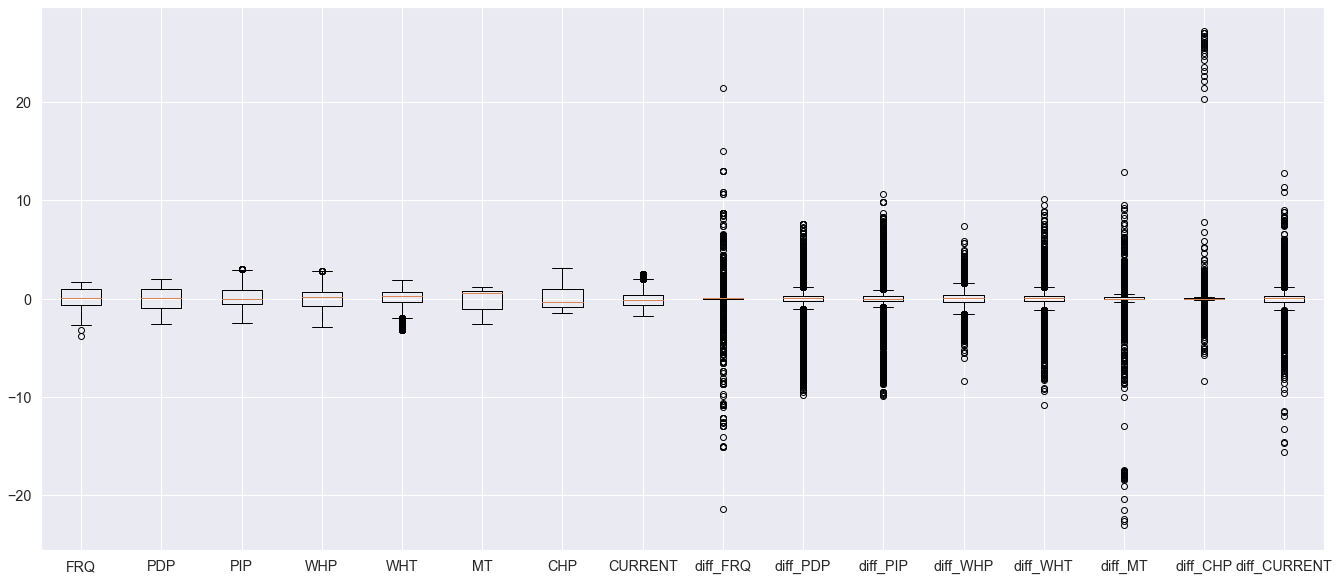
\includegraphics[width=\textwidth]{figures/predictive_maintenance/Fig 4-updated.png}
    \caption{Box-plot after outlier normalization}
    \label{fig:boxplot_after_normalization}
\end{figure}

Table \ref{tab:esp_eda} describes the main signals after outliers and zero production points are removed without standardization. Table \ref{tab:class_esp} shows the number of available data points after mapping the sensor data. These data points are classified, based on workover sheets, into “Normal data”, “Pre-workover”, and “Workover”. Pre-workover data are data points that are reported seven days before the workover day. Workover events are the data points made available on workover day.  

\begin{table}[]
\center
\resizebox{\textwidth}{!}{%
\begin{tabular}{l|S[round-mode = places]|S[round-mode = places]|S[round-mode = places]|S[round-mode = places]|S[round-mode = places]|S[round-mode = places]|S[round-mode = places]|S[round-mode = places]|}
\cline{2-9}
                          & \ac{FRQ}[Hz] & \ac{PDP}[Psi] & \ac{PIP}[Psi] & \ac{WHP} [Psi] & \ac{WHT}[$^\circ$F] & MT[$^\circ$F]  & \ac{CHP}[Psi] & \ac{Current} [A] \\ \hline
\multicolumn{1}{|l|}{mean} & 52.6806238 & 1522.96643 & 855.891601 & 642.207855 & 62.3826216 & 137.11823  & 922.12718  & 349.645672 \\ \hline
\multicolumn{1}{|l|}{std}  & 4.29171119 & 187.461024 & 211.079864 & 608.613357 & 11.487392  & 32.397163  & 1883.03087 & 86.9083859 \\ \hline
\multicolumn{1}{|l|}{min} & 35       & 1086.5156 & 610.456   & 194.059   & 60.545  & 120.626 & 0         & 101.5963    \\ \hline
\multicolumn{1}{|l|}{25\%} & 49.702205  & 1506.13425 & 660.900075 & 213.385671 & 63.231987  & 122.2008   & 91.5382681 & 317.009525 \\ \hline
\multicolumn{1}{|l|}{50\%} & 52.76629   & 1543.801   & 721.8032   & 243.580588 & 65.9961325 & 154.192608 & 261.378201 & 354.0059   \\ \hline
\multicolumn{1}{|l|}{75\%} & 56.58294   & 1595.04975 & 778.89995  & 547.3371   & 67.6575825 & 160.6      & 405.28695  & 394.737969 \\ \hline
\multicolumn{1}{|l|}{max}  & 64.964555  & 1893.238   & 1578.28725 & 845.8625   & 122.843    & 169.3002   & 986.7425   & 598.211    \\ \hline
\end{tabular}%
}
\caption{Data Exploration}
\label{tab:esp_eda}
\end{table}

\begin{table}[]
\center
\begin{tabular}{|l|l|}
\hline
Condition    & Reported Data Points \\ \hline
Normal       & 339,089              \\ \hline
Pre-Workover & 1728                 \\ \hline
Workover     & 288                  \\ \hline
\end{tabular}%
\caption{Data Points Classification}
\label{tab:class_esp}
\end{table}

\section{\ac{PCA} Application }
\ac{PCA} is defined as an unsupervised dimensionality reduction technique. It reduces large dimensionality data sets into lower dimensions called principle components. This happens while preserving as much information as possible. It makes use of the interdependence of original data to build a \ac{PCA} model. This results in reducing the dimension of production parameters by making the most of the linear combinations and by generating a new Principal Component space (PCs)

\subsection{\ac{PCA} Calculations}
The process of obtaining a \ac{PCA} model from a raw dataset is divided into four steps as follows:
Firstly, the covariance matrix $\sum$ of the whole dataset is computed. It is important to see whether there is a relationship between contributing features. Equation \ref{Eq:cov_matrix} is used to find the covariance between each pair of dataset columns. 

\begin{equation}\label{Eq:cov_matrix}
    \sum =\ \frac{1}{n-1}\sum_{i=1}^{n}{(X_{ij}-\widetilde{x_j})(X_{ik}-\widetilde{x_k})}
\end{equation}
\nomenclature{$\sum$}{Covariance}
\nomenclature{$a$}{sldldsm sldm l}

The second step is to calculate eigenvectors and corresponding eigenvalues. Let A be the covariance matrix that has been computed in the first step, $\nu$ a vector and $\lambda$ a scalar that satisfies $A\nu=\lambda\nu$, then $\lambda$ is the eigenvalue corresponding to eigenvector $\nu$ of A. This step is considered the calculation of the principal components of the data.

The third step is determining the number of principal components. The eigenvectors only define the directions of the new axis while the eigenvalues represent the variance of the data along the new feature axes. Therefore, we sort the eigenvectors based on the eigenvalues. Hence, a threshold is chosen on the eigenvalues and cut off is made on the eigenvectors to select the most informative lower dimensional subspace. In other words, Lower variance dimensions are omitted. This is because they possess the least information about the data’s distribution.

The Fourth step consists of transforming the samples into the new subspace. In this last step, the lower dimensional subspace $W$ is selected. In the current step, the dataset samples are transformed into this new subspace via the equation $Y = W^ \prime. X$ where $W^\prime$ is the transpose of the matrix W. In the following, two principal components are computed and the data points are reoriented onto the new subspace. Fig. \ref{fig:pca} shows the simple geometric meaning of \ac{PCA}.

\begin{figure}
    \centering
    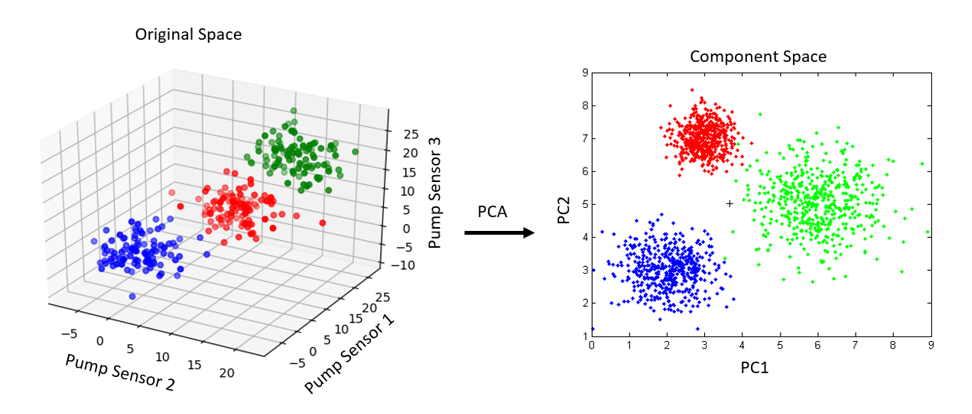
\includegraphics[keepaspectratio, width=\textwidth]{figures/predictive_maintenance/Fig 5.png}
    \caption{Geometric meaning of \ac{PCA}}
    \label{fig:pca}
\end{figure}

\subsection{Application of \ac{PCA} in the Electrical Submersible Pumps}
In ESP systems, sensor data are generally highly correlated, e.g., wellhead pressure is directly proportional to discharge and intake pressures. However, when a downhole problem occurs or is about to occur, anomalous data can be identified because it breaks certain rules in the input signals and their relative changes, i.e., if there is a tubing leak, the annulus discharge pressure decreases while intake pressure and annulus pressure increases, etc. 
Principal Component Analysis then suits the engineers’ purpose to create an anomaly detection system. This is mainly because it makes use of the interdependence of original data to build a model. The primary goal of this step is to create clusters out of the data.
As discussed earlier, the selection of the principal components is made based on the maximum variance criterion. The highest variance is captured in the first principal component while the next highest variance is captured in the second principal component, where information from the first principal component has already been removed. In a similar manner, consecutive principal components (3rd, 4th, ……, Kth) can be constructed to evaluate the original system. 
The PCA model finds the kth principal component to construct the PCs, where most of the information belonging to the initial system is contained. The kth principal component is represented in equation \ref{Eq:pcs} below where PC1 is given as an example.

\begin{equation}\label{Eq:pcs}
\begin{split}
    {PC}_k=a_{1k}\ast P_{intake\ pressure}+\ a_{2k}
    \ast P_{discarge\ pressure}+\ a_{3k}P_{Motor\ temperature}+\ldots \\
+a_{pk}P_{intake\ pressure\ moving\ difference}+..
\end{split}
\end{equation}

Figure \ref{fig:pca_esp} shows the projection of ESP well sensor data on the principal components. The developed model is used also to evaluate near failure conditions. The problematic days and seven days before workover, sensor data clearly show specific failure patterns in line with the reported \ac{MDHF} and \ac{EDHF}.

\begin{figure}
    \centering
    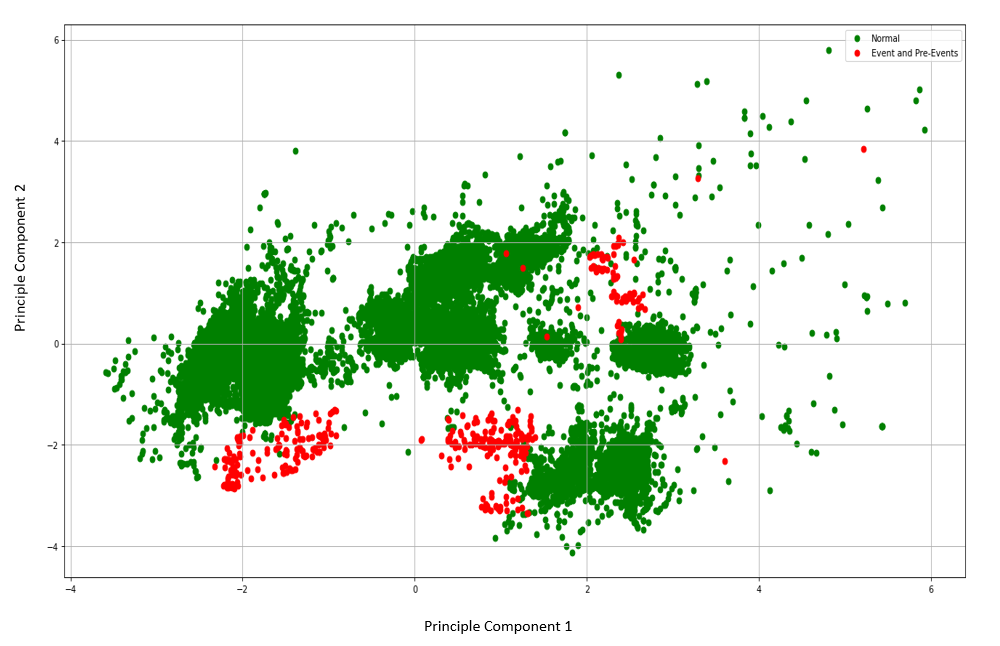
\includegraphics[keepaspectratio, width=\textwidth]{figures/predictive_maintenance/Fig 6.png}
    \caption{"Principle component analysis of ESP wells"}
    \label{fig:pca_esp}
\end{figure}

The goal of the \ac{PCA} is to come up with optimal weights from each sensor measurement. That means capturing as much information as possible from the input signals, based on the correlations among those variables. the loadings are the correlations between the variables and the component. We compute the weights in the weighted average from these loadings. To compute the Loading matrix, namely the correlations between the original variable and the principal components, the cross-covariance matrix is needed to be computed from equation \ref{Eq:cross_cov}.

\begin{equation}\label{Eq:cross_cov}
    Cov\left(X,\ Y\right)=V\sqrt E
\end{equation}

 Where: X is the original variables,
 	Y is the principal components,
 	V is the principal axes
E are its eigenvalues.
Table 4 represent the load factor for each input parameter in the relevant principle component till the 8th principle component. However, we mostly interested in parameters loading factors on the first and second principle component because they explain approximately 0.6 of the data variance as shown previously in figure 7. Large loadings (positive or negative) indicate that a particular variable has a strong relationship to a particular principal component. The sign of a loading indicates whether a variable and a principal component are positively or negatively correlated42. Hence, the most parameters correlated parameters with the first principle component are pump frequency, casing head pressure, current, motor temperature and well head temperature. 

% Please add the following required packages to your document preamble:
% \usepackage{graphicx}
\begin{table}[]
\resizebox{\textwidth}{!}{%
\begin{tabular}{|l|l|l|l|l|l|l|l|l|}
\hline
              & PC1   & PC2   & PC3   & PC4   & PC5   & PC6   & PC7   & PC8   \\ \hline
FRQ           & -0.90 & -0.05 & 0.06  & 0.05  & -0.05 & -0.26 & 0.05  & 0.01  \\ \hline
PDP           & -0.54 & -0.14 & -0.70 & 0.32  & -0.07 & -0.08 & 0.04  & 0.05  \\ \hline
PIP           & 0.03  & -0.17 & -0.47 & 0.14  & -0.05 & 0.81  & -0.18 & -0.04 \\ \hline
WHP           & 0.10  & -0.02 & -0.79 & 0.37  & -0.01 & -0.15 & 0.23  & -0.28 \\ \hline
WHT           & -0.63 & 0.00  & 0.35  & -0.30 & 0.18  & 0.22  & 0.12  & -0.32 \\ \hline
MT            & -0.79 & -0.12 & -0.07 & 0.04  & -0.12 & 0.25  & -0.16 & 0.22  \\ \hline
CHP           & -0.85 & -0.15 & -0.07 & 0.15  & -0.03 & -0.27 & 0.07  & 0.12  \\ \hline
CURRENT       & -0.84 & -0.10 & 0.21  & -0.17 & 0.07  & 0.21  & -0.06 & -0.19 \\ \hline
diff\_FRQ     & -0.14 & 0.78  & 0.03  & 0.27  & 0.09  & 0.02  & -0.22 & -0.17 \\ \hline
diff\_PDP     & -0.05 & 0.09  & -0.45 & -0.54 & 0.21  & -0.19 & -0.40 & 0.28  \\ \hline
diff\_PIP     & 0.06  & -0.35 & -0.34 & -0.67 & -0.21 & 0.06  & 0.18  & 0.11  \\ \hline
diff\_WHP     & -0.03 & 0.11  & -0.42 & -0.50 & 0.36  & -0.15 & -0.05 & -0.42 \\ \hline
diff\_WHT     & -0.10 & 0.43  & -0.08 & -0.11 & 0.37  & 0.23  & 0.69  & 0.26  \\ \hline
diff\_MT      & -0.15 & 0.84  & -0.10 & -0.10 & -0.34 & 0.03  & -0.03 & -0.03 \\ \hline
diff\_CHP     & 0.03  & -0.29 & 0.03  & 0.30  & 0.85  & 0.01  & -0.14 & 0.11  \\ \hline
diff\_CURRENT & -0.13 & 0.80  & -0.14 & -0.04 & 0.16  & 0.05  & -0.09 & 0.20  \\ \hline
\end{tabular}%
}
\caption{Loading for input parameters}
\label{input_loading_pca}
\end{table}


\section{\ac{XGBoosting} Application}
\ac{XGBoosting} is a tree-based ensemble model. Ensemble learning is a systematic solution that combines the predictive abilities of multiple models, eventually resulting in a single model. This single model provides the aggregated output of several models that, on their turn, only perform slightly better than random guessing. Therefore, Extreme Gradient Boosting (XGBoost) is an ensemble set of predictors, with a unified objective of predicting the same target variable. A final prediction is performed through the combination of these set of predictors.	
\subsection{\ac{XGBoosting} Calculations  }
Building an XGBoost model has the following sequence. It starts with a single root (contains all the training samples). Then, an iteration is performed over all features and values per feature and subsequently, each possible split loss reduction is evaluated. Equations 6 and 7 represent the objective function (loss function and regularization, respectively) at each iteration that is needed to be minimized.
\begin{equation}
\mathcal{L}^{\left(t\right)}=\ \sum_{i=1}^{n}{l\left(y_i,p_i+\ O_{value}\right)+\frac{1}{2}\lambda}O_{value}^2    
\end{equation}
\begin{equation}
    l\left(y_i,p_i\right)=-\left[y_i\log{\left(p_i\right)+\left(1-y_i\right)\log{\left(1-p_i\right)}}\right]
\end{equation}
Where: \\
$y_i$ is the true value required to be predicted of the i-th instance \\
$p_i$ is the prediction of the i-th instance\\
$\left(y_i,p_i\right)$ The loss function for typical classification problem \\
$O_{value}$ The output of the new tree\\
$\frac{1}{2}\lambda O_{value}^2$ Regularization Term\\

Tianqui stated “XGBoost objective function cannot be optimized using traditional optimization methods in Euclidean space”44. Therefore, in order to be able to transform this objective function to the Euclidean domain, the second-order Taylor approximation is used enabling traditional optimization techniques to be employed. Equation 8 and 9 represent the Taylor approximation of the loss function.

\begin{equation}
    \mathcal{L}^{(t)}\cong[\sum_{i=1}^{n}{l\left(y_i,p_i\right)+g_iO_{value}+\frac{1}{2}h_iO_{value}^2}]+\frac{1}{2}\lambda}O_{value}^2    
\end{equation}

Where: \\ 
$g_i$ is the gradient and calculated by $g_i=\ \frac{\partial}{\partial p_i}l(y_i,\ p_i)$  \\
$h_i$ is the hessian and calculated by $h_i=\ \frac{\partial^2}{\partial p_i^2}l(y_i,\ p_i)$ \\     	 	 	 	
Finally, removing the constant parts, the simplified objective to minimize at step t, results in:
\begin{equation}
    \mathcal{L}^{(t)}=\ \sum_{i=1}^{n}{g_iO_{value}+\frac{1}{2}h_iO_{value}^2+\frac{1}{2}\lambda O_{value}^2}		
\end{equation}

Equations 10 and 11 show how to minimize that function 

\begin{equation}
\frac{d}{dO_{value}}\ \sum_{i=1}^{n}{g_iO_{value}+\frac{1}{2}h_iO_{value}^2}+\frac{1}{2}\lambda O_{value}^2=0    
\end{equation}

\begin{equation}
    O_{value}=\ -\ \frac{\sum_{i=1}^{n}g_i}{\sum_{i}^{n}{h_i+\lambda}}					
\end{equation}

By combining equation 10 with the first and the second derivative of the classification loss function $g_i$ and $h_i$, the similarity equation is derived. The similarity score is calculated as follows in equation 12: 

\begin{equation}
    Similarity\ =\frac{\sum{Residual}_i}{\sum{{Previous\ Probability}_i\ast\ \left(1-{Previous\ Probability}_i\right)+\ \lambda}}\
\end{equation}

The similarity score is calculated for a “leaf” of the “tree”. Various thresholds are used to split the tree into more leaves. The similarity score is calculated for each new leaf followed by calculating the so-called gain as presented in equation 13 below: 

\begin{equation}
    Gain={Left}_{similarity}+{Right}_{similarity}-{Root}_{similarity}	
\end{equation}

Then thresholds continue to be set until higher gain thresholds are reached and the tree keeps growing. There is a minimum number of residuals in each leaf where the tree stops growing. This number is determined by calculating a parameter called cover. It is defined as the denominator of the similarity score minus lambda. During boosting, the operation is performed such that trees are sequentially constructed. Each tree reduces the error of its predecessor and learns from it while simultaneously updating the residual errors. As a result, each tree growing in the sequence will learn from a version of the residuals that’s already been updated. 

Further, in boosting, the base learners are weak due to their high bias and their predictive power has only a slight improvement over random guessing. Nevertheless, some vital information for prediction is supplied by each of these weak learners. By means of boosting, a strong learning effect is produced through combining these weak learners into a single strong learner that reduces both the bias and the variance.   
\subsection{XGBoosting Application}
In our proposed model, Principal Component Analysis (PCA) for sensor measurements and moving difference is pipelined with XGBoost and K-Folds Cross-validation to identify near failure regions. The dataset is divided into two groups: A training dataset containing 70 % of the data and a black box testing set with the remaining 30% of the data.

The importance of principal components is evident because it shows to which extent this component is able to explain the variance in the dataset. Therefore, Figure \ref{fig:explained_variance} shows the cumulative explained variance with each principal component. It is shown that 8 principle components will include more than 90% of the explained variance in the dataset of ESP sensors and their derived features. 

\begin{figure}
    \centering
    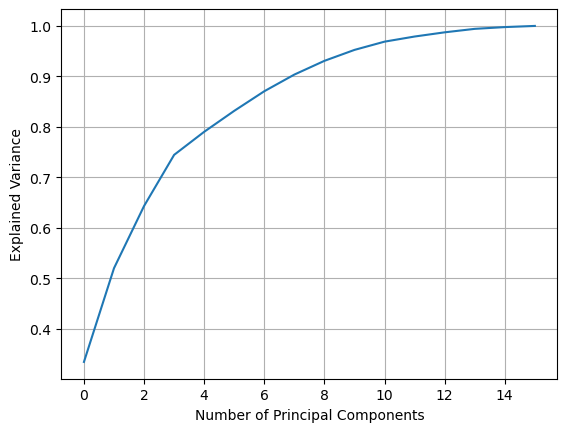
\includegraphics[keepaspectratio, width=\textwidth]{figures/predictive_maintenance/Fig 7-updated_2.png}
    \caption{Explained Variance of the proposed model}
    \label{fig:explained_variance}
\end{figure}

In the cross-validation algorithm, the data set is divided into 3 components as follows: a training set constituting 70% of the data, a validation set constituting 15% of the data and a testing set constituting the remaining 15% of the data. Each model is then trained on the training subset only, in order to infer some hypothesis. Finally, the hypothesis with the smallest error on the cross-validation set is selected.

A better estimation of each hypothesis is achieved through testing a set of examples (validation set) that the models were not trained on. A true generalization error is also obtained. As a consequence, a single model possessing the smallest estimated generalization error can be then proposed. Upon validation set error minimization, this can be further expanded such that the proposed model is retrained on the entire training set, including the validation set. It is worth noting that some risk exists in selecting validation points, which may contain a disproportionate amount of difficult and obscure examples. Therefore, the k-fold cross validation maybe applied to avoid such occurrences. 

A K-fold cross validation algorithm aims at selecting validation sets. initially, the dataset is randomly divided into (k) disjoint subsets. In each subset, the number of readings is equal to the total number of data points (m) over (k). These subsets are indicated by m1 to mk. Then, subset is evaluated for each model as follows:

All these subsets are used to train The XGBoost model, with the exception of the subset mj. The intention behind excluding this subset is to infer a hypothesis which is eventually tested on (mj). As such, the error of testing the hypothesis on the subset (mj) is calculated and the estimated generalization error of the model is calculated by averaging over (mj). Afterwards, the selection of the model with the lowest estimated generalization error is performed, and lastly the selected model is retained on the entire training set (m). The hypothesis resulting from such operation would be the final answer. When Performing cross validation, It is typically a standard that the chosen number of folds is equal to 10 (k=10)45.

Hyperparameter tuning is considered one of the important steps while creating any data driven model to get the best results from the deployed algorithm. Regarding the XGBoost Algorithm, hyper-parameters are divided into three categories. These categories are known as general parameters, booster parameters, and learning task parameters. 

General hyper-parameters define the type of algorithm to be either linear or tree based, the verbosity to print results and the number of threads to run on. Booster parameters include the main tuned parameters for the algorithms such as learning rate, the minimum sum of weights of all observations required in an internal node in the tree, and the learning parameters to specify the minimum loss reduction required to make a split46. These parameters are used to define the optimization objective and the metric to be calculated at each step. Table 5 shows ranges that are used for hyper-parameters tuning.

% Please add the following required packages to your document preamble:
% \usepackage{graphicx}
\begin{table}[]
\resizebox{\columnwidth}{!}{%
\begin{tabular}{|l|p{5cm}|l|l|}
\hline
Parameter         & Reference   to                                                          & Sampling   type         & range  \\ \hline
max\_depth &
  control   of over-fitting, higher depth facilitates such that the model learns   relations that are specific to a particular sample. &
  Suggest   integer value &
  2,10 \\ \hline
min\_child\_weight &
  a   minimum sum of weights is defined for all observations required in a child. &
  Log   uniform &
  1e-10, 1e10 \\ \hline
colsample\_bytree & The   subsample ratio of columns when constructing each tree.           & Uniform                 & 0, 1   \\ \hline
learning\_rate    & Overfitting   prevention through step size shrinkage in updates         & Uniform                 & 0, 0.1 \\ \hline
Gamma             & Specification of the minimum loss reduction required   to make a split. & Suggest   integer value & 0, 5   \\ \hline
\end{tabular}%
}
\caption{Hyper-parameters tuning}
\label{tab:xg_hyper}
\end{table}

\section{Validation and Testing}
Overfitting is a comparative term. It happens when learning algorithm tracking noise in input dataset instead of the underlying concept [52]. Therefore, the key point of overfitting is that the model fits the training data too much. However, it gives poor predictions with new data sets. It is often a result of complicated model. Overfitting can be prevented by validation and regularization those are called overfitting techniques. 

Overfitting occurs when input dataset error decreases parallel with increase in testing dataset error. While training, the input error goes down. This is good when it is associated with testing error reduction.  The problem happens when input error decreases while testing error increases. It is thought that the algorithm performance is well. However, it is actually harming the performance.

Overfitting techniques were applied to almost any machine learning problem. They are applied on top of any algorithm or model such as Artificial Neural Networks or Support Vector Machine. Therefore, this is another layer of techniques for machine learning. These techniques are regularization and validation [53]. 

Regularization can be considered as if it puts brakes on fitting the noise. Hard and soft constraints may be used. Validation detects the maximum number of iterations to adjust the classifier. It is the determination of a stopping point for the back-propagation algorithm [54].

In cross validation algorithm, first, randomly split dataset into training set (70% of the data), validation set (15% of the data) and testing set (15% of the data). Then, each model is trained on the training set only, to get some hypothesis. Finally, the hypothesis is selected (that had the smallest error on the cross validation set).
 
By testing on a set of examples (validation set) that the models were not trained on. A better estimation of each hypothesis is achieved. Also, true generalization error is obtained. Simply, one with the smallest estimated generalization error can be then proposed.

Optionally, after selecting model according to minimizing error in validation set. Then, the proposed model is retrained on the entire training set including validation set. 

There is also some risk in the selection of validation points. The validation set may contain a disproportionate number of difficult or obscure examples. To combat this,
k-fold cross validation can be performed.

K-fold cross validation algorithm is used to select validation sets. First, randomly the dataset is split into (k) disjoint subsets. The number of examples in each subset is equal to total number of data examples (m) over (k) [56]. These subsets are referred to as m1 to mk. Then for each model, it is evaluated as follows:

The model is trained for all subsets except one of this subsets $(m_j)$ to get some hypothesis.

The hypothesis is tested on $(m_j)$. Then error of testing over $(m_j)$ is calculated. The estimated generalization error of model is then calculated as the average over $(m_j)$.

The model is picked with the lowest estimated generalization error. Finally, the model is retrained on the entire training set (m). The resulting hypothesis is then output as a final answer. A typical choice for the number of folds to use would be k = 10. Fig. 4.11 shows 10-fold cross-validation.

After running experiments, it is important to inspect the evaluation results. Then, the various models’ results are compared. At the end, the most accurate and generalized results are chosen.   

The accuracy for each scenario or each model is based on how many outputs are correctly classified out of all testing samples [57]. Therefore, the accuracy would be calculated as shown in Equation 4.37.  

After choosing the best model, the classifier output quality is evaluated. The accuracy is simply the proportion of correctly classified instances. It is usually the first metric when evaluating a classifier. However, what if the test data is unbalanced? In the other words, the most of the instances belongs to one of the classes. The accuracy doesn’t really capture the effectiveness of a classifier at that case [58]. 

In the technical level classification scenario, it is assumed that the testing set includes 99% of the dynamometer cards of fluid pound problem. It is possible to achieve 99% accuracy by predicting the class “fluid pound” for all instances. The classifier in this case appears to be doing a good job overall. However, it fails to classify any of the rod pumping conditions (1%) correctly.

For that reason, it is helpful to compute additional metrics that capture more specific aspects of the evaluation. Before going into the details of such metrics, it is important to understand the confusion matrix of a binary classification evaluation. The class labels in the training set can take on only two possible values. These two values always take positive or negative. The positive and negative instances that a classifier predicts correctly are called true positives (TP) and true negatives (TN), respectively. Similarly, the incorrectly classified instances are called false positives (FP) and false negatives (FN). Fig. 4.12 shows the confusion matrix. The confusion matrix is simply a table showing the number of instances that fall under each of these four categories. 

Fig. 4.12-Confussion Matrix
Understanding the performance of the classifier requires answering some important questions. A very natural question is: ‘Out of the dynamometer classified as specific condition, how many were classified correctly?’ This question can be answered by looking at the Precision of the model.  The Precision is the proportion of the positives that are classified correctly [58]. Equation 4.39 is the mathematical form of the Precision: 
\begin{equation}
    Precision=\ \frac{True\ Positive}{True\ Positive+False\ positive}\ldots\ldots\ldots\ldots\ldots\ldots\ldots\ldots\ldots
 \end{equation}
   
Another common question is “Out of all cards having specific condition (TP+FN), how many did the classifier classify correctly (TP)?” This is actually the Recall, or the true positive rate [56]. Equation 4.40 is the mathematical form of the Recall:

\begin{equation}
     Recall=\ \frac{True\ Positive}{True\ Positive+False\ Negative}\ldots\ldots\ldots\ldots\ldots\ldots\ldots\ldots\ldots   
\end{equation}
    

To conclude, the Precision-Recall metric is an important tool to evaluate the classifier output quality. Precision is a measure of how good predictions are with regard to false positives. Recall is also known as sensitivity or true positive rate. It measures how good the predictions are with regard to false negatives.

3.1- Evaluation Metrics
Some questions are vital for understanding the classifier performance. One of which is the number of signals that have been classified correctly among the entirety of those that have been classified as “Pre-workover”. The answer lies in inspecting the model’s precision. Precision is the ratio of positives that have been correctly classified to the sum of both positives and negatives. This is the percent of the true alarms which is an important measure to eliminate the false pre-workover alarms as much as possible.
Precision = True Positive / (True Positive + False Positive)40
Another common question is the proportion of correctly classified Pre-workover signals (TP) to the total Pre-workover signals (TP+FN) that are identifiable and non-identifiable by the model. This is the Recall, or the true positive rate which indicates how capable the model is of finding the Pre-workover signals.
Recall = True Positive / (True Positive + False negative)40
The F1-score is the harmonic mean of the precision and recall. F1 score is used for model validation. F-measure has an intuitive meaning. It describes how precise our classifier is (how many events are classified correctly), as well as how robust it is, i.e. not missing a significant number of events.
3.2 Diagnostic Tools
A receiver operating characteristic curve (ROC) is applied as a diagnostic tool where the performance of a classification model is summarized with respect to the positive class. The False Positive Rate is the x-axis and the True Positive Rate is the y-axis.
The true positive rate is the ratio of the total number of true positive predictions to the sum of the true positives and the false negatives (e.g., all examples in the positive class). The true positive rate is referred to as the sensitivity or the recall.
True Positive Rate = True Positives / (True Positives + False Negatives)
The false positive rate is the ratio of the total number of false positive predictions to the sum of the false positives and true negatives (e.g., all examples in the negative class)46.
False Positive Rate = False Positives / (False Positives + True Negatives)


\section{summary}
In this application, sensors measurements with moving difference is applied to the dataset in order to predict pumping condition. Then a dimensionality reduction technique is used and the whole dataset points have been projected to the new lower dimensions. Finally, these new transformed data have been pipelined with supervised algorithm, which is XGBoosting in our application. The training dataset consists of inputs (PCA projected features) paired with the representative outputs (in case of ESP failure prediction, the labelled outputs are the seven days before the reported failures). Each of these inputs-output pairs should be seen as a “data point” that can be used to train, validate and test the proposed model. 

Regarding validation set, the proposed model has a mean AUC for the 10-fold validation equal to 0.95. which in turn means that the model has an adequate performance and can be tested on the upcoming processes against test sets. 

Regarding testing sets, the proposed model can report the pre-workover and workover class with 0.8 precision and 0.6 recall. The model has high precision on testing sets and hence a small number of false alarms. Of course, the relevant recall is small, which means not all the 7 days before the event are marked as yellow alarm (pre-workover and workover event). In other words, the model will report alarms with high precision but not for all days before the workover, which is acceptable because it is not necessary that all days before the event will exhibit a sign of an upcoming workover.     
